\author{Josef Stieg}

\section{Zielgruppe}

\textit{Melius} adressiert Personen aus der IT- und der kreativen Branche, die auf der Suche nach einer neuen beruflichen Herausforderung sind oder ihre beruflichen Kompetenzen auf attraktive Weise präsentieren möchten. Gleichzeitig bietet die Plattform Unternehmen aus diesen Bereichen die Möglichkeit, mithilfe der Gruppenfunktion ihre Teammitglieder basierend auf deren Stärken und Kompetenzen effizient und übersichtlich zu filtern. Die Nutzung von \textit{Melius} ist nicht auf eine bestimmte Altersgruppe beschränkt, sodass sowohl Berufseinsteiger als auch erfahrene Fachkräfte von den Funktionen profitieren können.

\subsection{Bedarf}

\textit{Melius} adressiert eine zentrale Problematik im Bewerbungsprozess, die sich aus der umständlichen und oft speicherplatzbegrenzten Übermittlung von Portfolios in Form mehrerer einzelner Dateien ergibt. Anstatt Bewerbungen mit zahlreichen Anhängen zu verschicken, ermöglicht \textit{Melius} eine kompakte und übersichtliche Darstellung aller relevanten Inhalte – von Lebenslauf und Kompetenzen bis hin zu Projekten und Bildern – auf einer einzigen, personalisierten Portfolio-Seite. Für Bewerber reduziert sich der Aufwand auf das Teilen eines Links, was die Notwendigkeit betrifft, mit Datei-Limits und unübersichtlichen Anhängen zu arbeiten.

Die Gruppenfunktion von \textit{Melius} bietet Unternehmen und Teams eine wertvolle Unterstützung. Innerhalb einer Gruppe können alle Mitglieder die Profile der anderen einsehen und gezielt nach bestimmten Fähigkeiten filtern. Dies ermöglicht es nicht nur Personalverantwortlichen, sondern auch den Mitarbeitenden selbst, schnell und einfach die richtige Person für eine Aufgabe oder ein Projekt zu finden. Die Effizienz der Zusammenarbeit wird gesteigert und das vorhandene Know-how innerhalb eines Teams besser genutzt.

\section{Ähnliche Online - Portfolio Plattformen}

\subsection{Pixpa}

Pixpa ist eine All-in-One-Plattform, die es Kreativen und kleinen Unternehmen ermöglicht, professionelle Portfolio-Websites zu erstellen, ohne über Programmierkenntnisse zu verfügen. Der benutzerfreundliche Drag-and-Drop-Editor und die über 200 anpassbaren, responsiven Vorlagen ermöglichen es den Nutzern, ihre Arbeiten ansprechend zu präsentieren. Darüber hinaus umfasst Pixpa integrierte Funktionen wie E-Commerce, Blogging, SEO- und Marketing-Tools sowie Kundengalerien und stellt somit eine umfassende Lösung für die Online-Präsenz bereit.Die Kosten für die Nutzung der Plattform betragen ab 3,60 USD pro Monat bei einer zweijährlichen Abrechnungsperiode.

\begin{figure}[H]
    \centering
    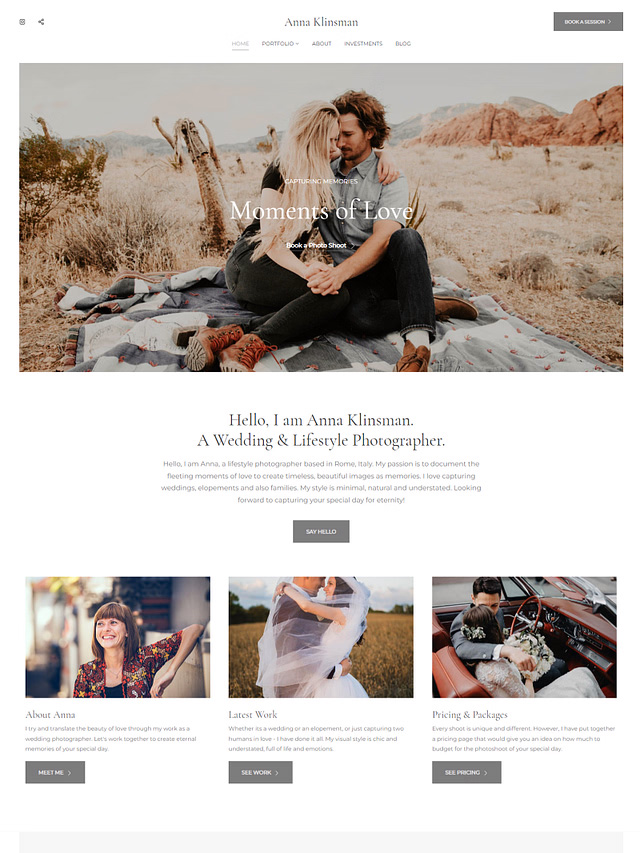
\includegraphics[width=0.5\linewidth]{pics/Umfeldanalyse/pixpa.jpg}
    \caption{Pixpa - Portfolio}
    \label{fig:entities}
\end{figure}

\subsection{Canva}

Canva ist für seine benutzerfreundliche Design-Plattform bekannt und bietet auch eine einfache Möglichkeit, Portfolio-Websites zu erstellen. Mit einer Vielzahl von Vorlagen und einem intuitiven Editor können Nutzer ohne Vorkenntnisse schnell ansprechende Portfolios gestalten. Canva eignet sich besonders für Anfänger, die eine unkomplizierte Lösung suchen, um ihre Arbeiten online zu präsentieren.

\begin{figure}[H]
    \centering
    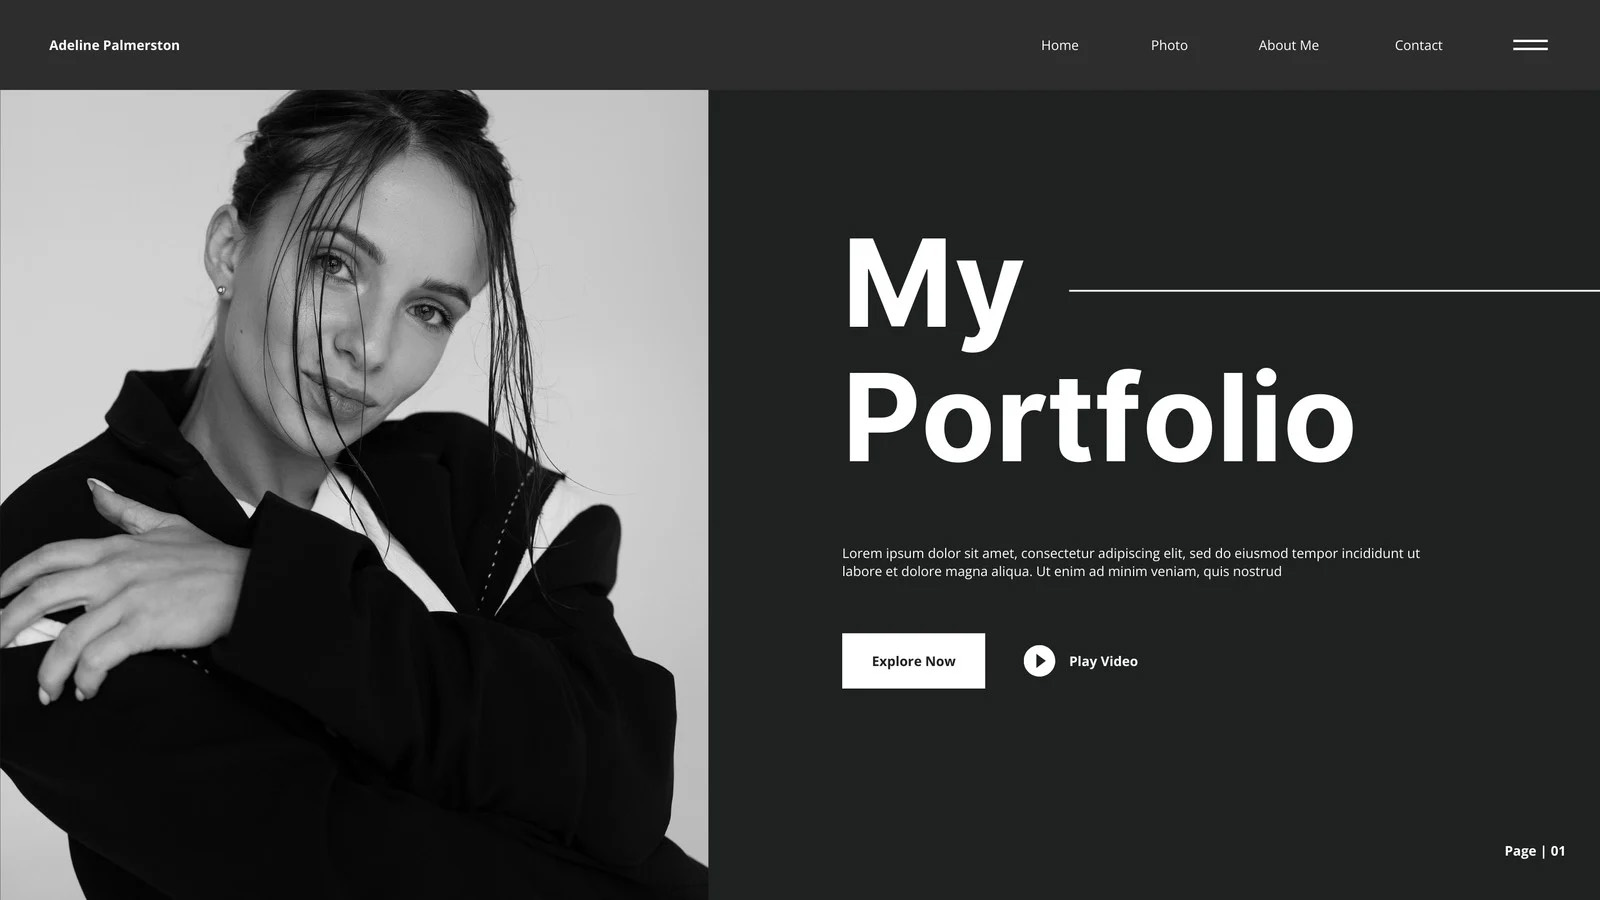
\includegraphics[width=0.5\linewidth]{pics/Umfeldanalyse/Canva.jpg}
    \caption{Canva - Portfolio}
    \label{fig:entities}
\end{figure}

\subsection{Adobe Portfolio}

Adobe Portfolio ist ein Element der Adobe Creative Cloud und ermöglicht es professionellen Kreativschaffenden, nahtlos Portfolio-Websites zu erstellen, die eine Integration mit anderen Adobe-Produkten erlauben. Mithilfe einer Auswahl an modernen, responsiven Vorlagen können Nutzer ihre Arbeiten stilvoll präsentieren. Adobe Portfolio ist ideal für diejenigen, die bereits andere Adobe-Tools verwenden und eine kohärente Plattform für ihre Projekte wünschen.

\begin{figure}[H]
    \centering
    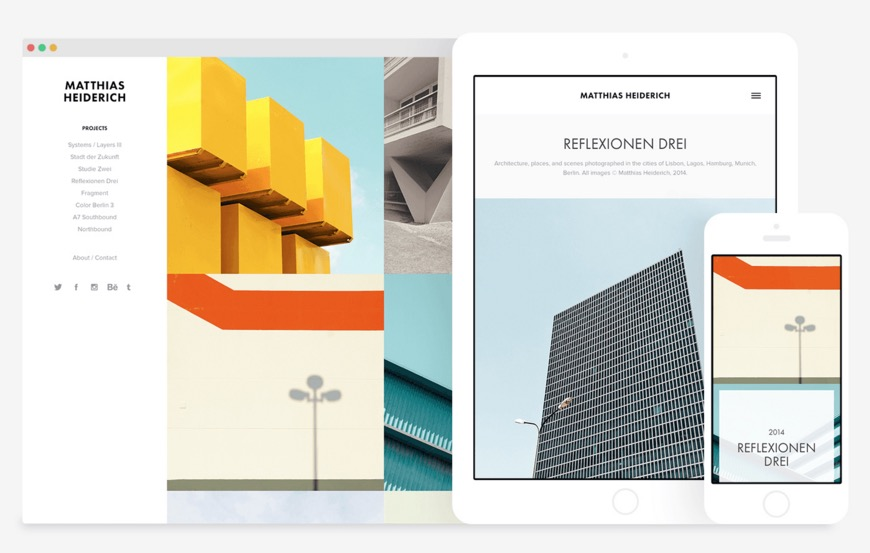
\includegraphics[width=0.5\linewidth]{pics/Umfeldanalyse/adobe.jpg}
    \caption{Adobe - Portfolio}
    \label{fig:entities}
\end{figure}

\subsection{Squarespace}

Squarespace stellt eine Vielzahl von professionell gestalteten Vorlagen bereit, die insbesondere für Designer geeignet sind. Ein leistungsstarker Editor und umfangreiche Anpassungsmöglichkeiten ermöglichen es den Nutzern, individuelle Portfolio-Websites zu erstellen. Darüber hinaus bietet Squarespace Funktionen wie Blogging, E-Commerce und SEO-Tools, um die Online-Präsenz zu stärken.

\begin{figure}[H]
    \centering
    
\includegraphics[width=0.5\linewidth]{pics/Umfeldanalyse/squarespace.jpg}
    \caption{Squarespace - Portfolio}
    \label{fig:entities}
\end{figure}

\subsection{Wix}

Wix ist für seine Flexibilität bekannt und bietet eine große Auswahl an Vorlagen sowie einen intuitiven Drag-and-Drop-Editor. Nutzer können ihre Portfolio-Websites nach ihren Vorstellungen gestalten und von zahlreichen Apps und Integrationen profitieren. Wix eignet sich für Personen, die eine anpassbare Lösung suchen, um ihre Arbeiten online zu präsentieren.

\begin{figure}[H]
    \centering
    
\includegraphics[width=0.5\linewidth]{pics/Umfeldanalyse/wix.jpg}
    \caption{Wix - Portfolio}
    \label{fig:entities}
\end{figure}

\subsection{Vergleich mit Melius}

\textit{Melius} bietet einige einzigartige Funktionen, die es von anderen bekannten Portfolio-Website-Buildern wie Pixpa, Canva, Adobe Portfolio, Squarespace und Wix abheben. Ein besonders hervorstechendes Merkmal ist die Gruppenfunktion, die es Unternehmen ermöglicht, ihre Mitarbeiter oder Kollegen zu organisieren und nach spezifischen Kompetenzen zu filtern. Diese Funktion ist besonders nützlich für Personalabteilungen, die eine detaillierte Übersicht über die Fähigkeiten ihrer Mitarbeiter benötigen, was bei den anderen Plattformen nicht der Fall ist.

Ein weiterer Vorteil von \textit{Melius} ist der spezifische Fokus auf die IT- und kreative Branche. Während viele andere Tools allgemein für kreative Berufe entwickelt wurden, richtet sich Melius speziell an IT-Profis und kreative Fachkräfte und ermöglicht es, Projekte wie GitHub-Repositories oder technische Arbeiten direkt in das Portfolio zu integrieren.

\textit{Melius} bietet außerdem eine tiefere Backend-Integration und Datenbankfunktionen, die über einfache visuelle Designoptionen hinausgehen. Nutzer können ihre Portfolios und Bewerbungsunterlagen in einer strukturierten Weise verwalten, was bei den anderen Plattformen meist nicht der Fall ist, da diese sich vor allem auf Frontend-Design und Präsentation konzentrieren.

Schließlich ermöglicht \textit{Melius} eine zentralisierte Verwaltung von Lebensläufen, Projekten und Kompetenzen an einem Ort. Dies erleichtert die Erstellung und Verwaltung von Bewerbungsmaterialien erheblich, während andere Plattformen in der Regel auf die Gestaltung und Präsentation des Portfolios fokussiert sind, ohne diese integrierten Verwaltungstools zu bieten.

Dank dieser einzigartigen Funktionen stellt \textit{Melius} eine umfassendere und spezialisierten Lösung für IT-Profis und Kreative dar und hebt sich so von den traditionellen Portfolio-Website-Buildern ab.


